\newcommand{\COURSE}{Seminar: OPT/NAS 20/21}
\newcommand{\STUDENT}{Stefan Wezel}

\documentclass[a4paper]{scrartcl}

\usepackage[utf8]{inputenc}
\usepackage[ngerman]{babel}
\usepackage{amsmath}
\usepackage{amssymb}
\usepackage{fancyhdr}
\usepackage{color}
%\usepackage{natbib}
\usepackage{graphicx}
\usepackage{lastpage}
\usepackage{listings}
\usepackage{tikz}
\usepackage{pdflscape}
\usepackage{subfigure}
\usepackage{float}
\usepackage{polynom}
\usepackage{hyperref}
\usepackage{tabularx}
\usepackage{forloop}
\usepackage{geometry}
\usepackage{listings}
\usepackage{fancybox}
\usepackage{tikz}
\usepackage{algpseudocode,algorithm,algorithmicx}

%Definiere Let-Command für algorithmen
\newcommand*\Let[2]{\State #1 $\gets$ #2}

\input kvmacros

%Größe der Ränder setzen
\geometry{a4paper,left=3cm, right=3cm, top=3cm, bottom=3cm}


\bibliographystyle{apalike}	% lengthly
%Kopf- und Fußzeile
\pagestyle {fancy}
\fancyhead[L]{\STUDENT}
\fancyhead[C]{\COURSE}
\fancyhead[R]{\today}

\fancyfoot[L]{}
\fancyfoot[C]{}
\fancyfoot[R]{Page \thepage /\pageref*{LastPage}}
\title{\textbf{Loss Landscape Visualization}\\\small Report for the Seminar on Optimization and Neural Architecture Search}
\author{Stefan Wezel}


\begin{document}	
	
	
	% ----------------------- TODO ---------------------------
	% Hier werden die Aufgaben/Lösungen eingetragen:

%\author{Stefan Wezel}	
\maketitle
%\tableofcontents


	% TODO remove sample text

\section*{Abstract}
\textit{Neural networks have emerged as powerful function approximators with large parameter sets. These parameters are optimized according to a loss function. Many assumptions have been made about the shape of the resulting loss landscape. However, only recently qualitative and empricial studies have been conducted. Here, we give an overview for recent advances of this field. We will explore different methods in detail and discuss their results and impact.}



\section*{Introduction}
When creating neural networks for a given task, practicioners or have to take many decisions. From architecture design, over optimizers, and schedules to hyperparameter choice there are many options that will play a key role in the eventual performance of the model. Anecdotal knowledge, experience and luck often lead to the final configuration and there is little empirical knowledge of what is actually effective. Loss landscape visualization can play a large role in guiding the community towards a more empirically foundation and maybe help build the groundwork for theoretical approaches.\\
Several recent works have shown that a better knowledge about the loss landscape can help build methods grounded in theory \cite{mutschler2020parabolic, chaudhari2019entropy}. Moreover, loss landscape visualization also helped to explain the effectiveness of existing methods such as stochastic gradient descent (SGD) \cite{robbins1951stochastic, xing2018walk} and architectures with residual connections \cite{he2016deep, li2017visualizing}.\\
As the space of parameters is too large to visualize in any meaningful way, methods of loss landscape visualization have to compromise. They might just consider small, visualizable subspace of a model's parameters. Results, thus, should be considered with caution and any conclusions should be drawn only carefully.\\
The following section will give .. to deep neural network architectures, and explain what a loss landscape is. Then, we will explore different methods of visualizing loss landscapes and see how insights from those methods can be applied. Finally, we discuss the impact of knowing the loss landscape better, see some limitations, and give an outlook on the future of the field.



\section*{Background}
In this section we will provide some theoretical background and set the denotations for the following sections.\\
A neural network $g$ is a function with a set of adjustable parameters $\theta_i$. We will denote it by $g_{\theta_i}$. Deep neural networks (DNN) can be viewed as the composition $f_{\theta} = \sigma (g_{\theta_0}) \circ ... \circ \sigma(g_{\theta_m})$ of such functions where $\sigma$ denotes some non-linear function. The parameter set $\theta$ may be arbitrary. For a given task it can be optimized by finding a minimum of a loss function $\mathcal{L}$. We refer to the resulting set as $\theta^*$. Du to the non-linear functions involved and the often large magnitude of $\theta$ a solution usually cannot be found analytically.\\
In recent years, however, iterative, algorithmic approaches have proven to reliably find sufficient minima. These approaches built on the notion of a gradient descient which dates back to \cite{cauchy1847methode}. A gradient according to the current loss $L$ and parameters $\theta_t$ is computed and a step, scaled by constant $\eta$ is taken in its negative direction. The result of a step taken is an adjusted set of parameters $\theta_{t+1}$. Note that for the gradient to be tractable, all operations involved have to be differentiable. Popular variants of the basic gradient descent algorithms include Stochastic Gradient Descent (SGD) \cite{robbins1951stochastic}, ADAM \cite{kingma2014adam}, and RMSProp \cite{graves2013generating}.\\
We refer to the surface, such an algorithm is moving on, as loss landscape. The dimension $n$ of the surface is determined by the magnitude of $\theta$. For $n=2$ this surface is easy to visualize as shown in Figure \ref{fig:twoweights}.

\label{fig:twoweights}
\begin{figure}
	\centering
	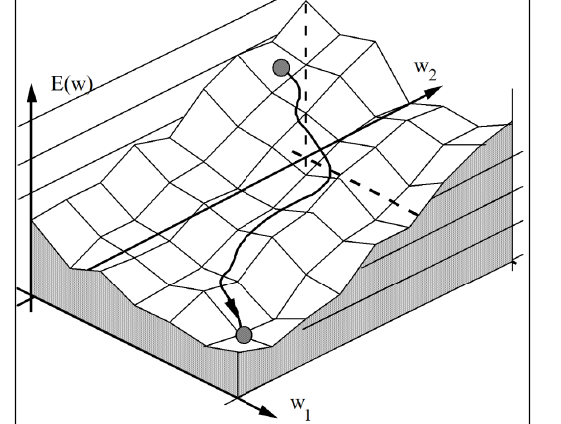
\includegraphics[width=.5\linewidth]{figures/two_weight_loss.png}
	\caption{Loss landscape for a neural network with $\theta = \lbrace w_1, w_2 \rbrace$. Values for $w_1, w_2$ are plotted against a loss $\mathcal{L}(\theta)$. As $|\theta| = 2$, visualization is straight forward.}
\end{figure}


It is often assumed that the path such an algorithm has to take in order to find a minimum encounters several obstacles and is highly non-convex. Recent insights from loss landscape visualization have, however, shown that this is highly dependent on the architecture. \cite{li2017visualizing} have shown that loss surfaces of architectures with residual connections can have roughly convex subspaces.\\
Another common assumption is that flat minima generalize better. The intuition behind this is that there might be a shift between train and test distribution. Thus, for a flatter minimum, the probability of also covering the test distribution would be higher. However this claim was lacking empirical or theoretical studies. Recently, loss landscape visualization has helped providing compelling evidence to support such claims.



\section*{Inspecting the Loss Landscape}
With the context set and some background, we can now have a look at approaches to visualize the high-dimensional loss landscape. The section \ref{subs:linear} will explore the rather simple technique of linear interpolation as proposed by \cite{goodfellow2014qualitatively}. A refined approach is taken by \cite{li2017visualizing} which will be described in section \ref{subs:filter}.


\label{subs:linear}
\subsection*{Linear Interpolation}
\cite{goodfellow2014qualitatively} propose to use a linear interpolation between two parameter sets $\theta_0$ and $\theta_1$ as visualizeable subspace. They plot the function shown in Equation \ref{eq:linear} where $\mathcal{L}$ is the loss function and $\alpha$ serves as weighting parameter. The scalar $\alpha$ can for example be in a range of $0$ to $1$, thus ranging from full weight on model $\theta_0$ to interpolating towards full weigh on model $\theta_1$.
\label{eq:linear}
\begin{align}
	f(\alpha) &= \mathcal{L}((1-\alpha) \theta_0 + \alpha \theta_1)
\end{align}
The aussagekraft of such visualizations depends of course heavily on the choice of $\theta_0$ and $\theta_1$. Figure \ref{fig:untrained_trained} shows shows the interpolation between an untrained model $\theta_{untrained}$ and a model $\theta_{trained}$ trained for an image classification task.


\label{fig:untrained_trained}
\begin{figure}[H]
	\centering
	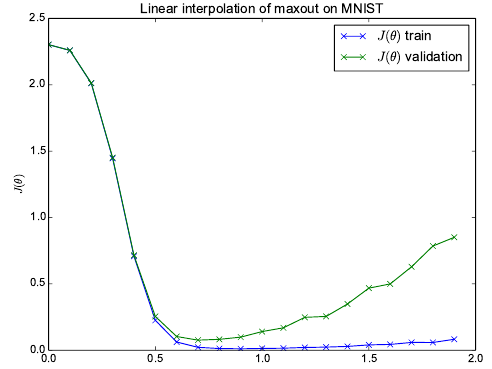
\includegraphics[width=.5\linewidth]{figures/linear_interpol_1.png}
	\caption{Linear interpolation between an untrained and a trained model.}
\end{figure}
The subspace visualized in this figure smoothly transitions between the two models and appears roughly convex.\\
\cite{li2017visualizing} use this technique to explore the effect of batch size in training on the shape of minima. A result is shown in Figure \ref{fig:smallbatch_largebatch}. When $\alpha =0$, meaning full weight is on the model trained with a small batch size the minimum is flat and wide. As $\alpha$ increases, the loss gets higher before it sharply drops into another minima, where full weight is on the model trained with a large batch size. This minimum is much sharper, indicating a relationship between batch size and flatness of an optimum. If the assumption that flat minima generalize better holds, this would render smaller batch sizes more favorable.
\label{fig:smallbatch_largebatch}
\begin{figure}[H]
	\centering
	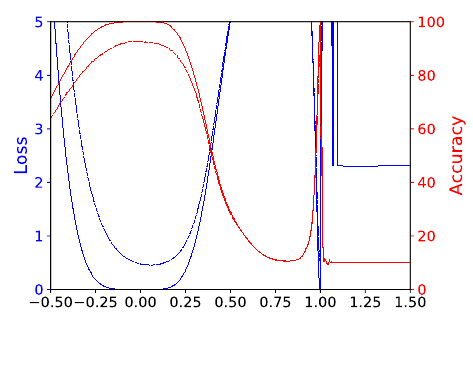
\includegraphics[width=.5\linewidth]{figures/batch_size_1.png}
	\caption{Linear interpolation between a model trained with a small batch size (left) and a model trained with a large batch size (right).}
\end{figure}

As discussed by \cite{li2017visualizing}, linear interpolation suffers from several shortcomings  and limitations. For example, it is arguable whether it is actually possible to capture non-convexities with this method. They thus propose to use filter normalization when visualizing loss landscapes. We will discuss their proposed methods and results in Section \ref{subs:filter}.



\label{subs:filter}
\subsection*{Filter Normalization}
Addressing the issues of \cite{goodfellow2014qualitatively}'s visualizations using plain linear interpolation, \cite{li2017visualizing} propose to scale normalized parameters $\theta$. For their method, rather than interpolating between two models, inspect the neighborhood around a model $\hat{\theta}$ by adding a direction vector $u$  of the same shape to $\hat{\theta}$. This direction vector is then scaled by different values for $\alpha$ and the corresponding loss is evaluated, yielding the equation
\begin{align*}
	f(\alpha) = \mathcal{L}(\hat{\theta} + \alpha u).
\end{align*}
To ensure that the updates along $u$ live on the same scale as the the values of $\hat{\theta}$, \cite{li2017visualizing} propose to normalize $u$ by setting
\begin{align}
	u = \frac{||\hat{\theta}||}{||u||},
\end{align}

thus normalizing the parameters of the neighborhood models. They propose the term filter normalization as they conduct most of their experiments on convolutional neural networks, where the most of $\hat{\theta}$ is use to parameterize filters.\\
\label{fig:smallbatch_largebatch_normalized}
\begin{figure}[H]
	\centering
	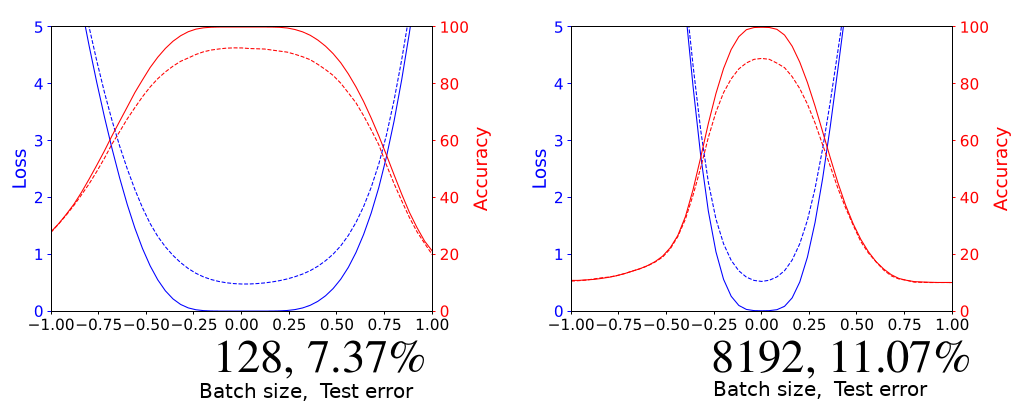
\includegraphics[width=.7\linewidth]{figures/batch_size_normalized.png}
	\caption{Loss landscape neighborhood around a model trained with a small batch size(left) and a model trained with a larger batch size.}
\end{figure}
Related to Figure \ref{fig:smallbatch_largebatch}, they visualize the filter normalized landscape around a model trained with a small batch size and a model trained with a large batch size. The result is shown in Figure \ref{fig:smallbatch_largebatch_normalized}. While a difference in flatness remains, it is much less clear with both models laying in rather flat minima. The minimum of the small batch size model is, however, still noticeably flatter. The resulting test error is also lower. This further hints towards a better generalization of flat minima and the batch size's role in finding such.\\
\cite{li2017visualizing} further expand this approach beyond 1-dimensional plots. By choosing not one but multiple direction vectors $u_i$, it can be used for higher dimensions. However, any dimension beyond two would result in the same dilemma for which such methods were developed. Thus, applying it to two dimensions is useful. The function to plot is then
\begin{align*}
		f(\alpha, \beta) = \mathcal{L}(\hat{\theta} + \alpha u_1 + \beta u_2).
\end{align*}
This results in more expressive plots, revealing more information about the $\hat{\theta}$'s neighborhood. An insightful example is given in Figure \ref{fig:2dloss} where two architectural paradigms are compared. 
\label{fig:2dloss}
\begin{figure}[H]
	\centering
	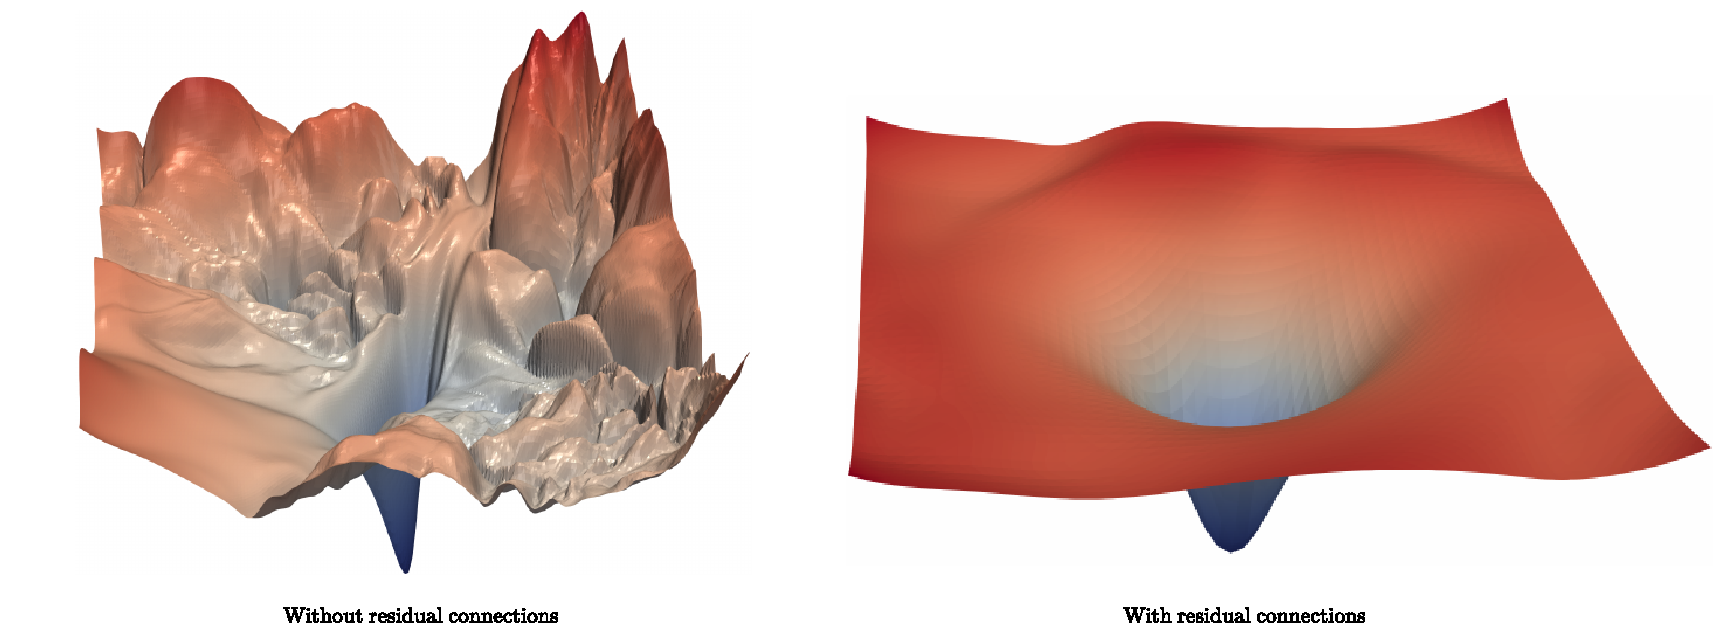
\includegraphics[width=\linewidth]{figures/2dloss.pdf}
	\caption{Loss landscape neighborhood around a model trained with a small batch size(left) and a model trained with a larger batch size.}
\end{figure}
The loss landscape around a minimum found with a model without any residual connections has several local minima. Intuitively put, an algorithm such as SGD might have a hard time traversing such rugged terrain. On the other hand, introducing residual connection results in a much smoother loss landscape around the minimum. It even appears roughly convex, in the visualized subspace.\\
While the methods proposed by \cite{li2017visualizing} produce more nuanced plots than simple linear interpolation, it is still important to mention that only a small subspace of the high dimensional parameter space is depicted. Thus, any conclusion has to be drawn with caution. It is also worth mentioning that their proposed method comes with high computational costs, as they consider the whole dataset to evaluate the empirical loss $\mathcal{L}$ at any considered point around $\hat{\theta}$. This 
severely limits the applicability of such methods. For reasonable experiments, only as small patch of neighborhood can be considered. Also the variety of currently existing architectures expands beyond just using residual connections or not. Moreover, this makes it also only usable with constraints for exploring the effect of different values for hyperparameters on the loss landscape.









\section*{Applying Findings from Loss Landscape Visualization}
\subsection*{Parabolic Approximation Line Search}
\subsection*{Entropy-SGD}


\section*{Conclusions}

\bibliographystyle{alpha}
\bibliography{references}

	
\end{document}
%%% Local Variables:
%%% mode: latex
%%% TeX-master: t
%%% End: